\documentclass[12pt]{article}   %  [titlepage]   \and
\usepackage{amsmath}
\usepackage[utf8]{inputenc}
\usepackage[T1]{fontenc}
\usepackage[danish]{babel}
\renewcommand{\rmdefault}{ptm}
\usepackage[pdftex]{graphicx}
\usepackage{multirow}
\newcommand{\nextitem}{\par\hspace*{\labelsep}\textbullet\hspace*{\labelsep}}

\title{Kalender og aftalebooking til K. Translation}
\author{Omar  - [26-10-87]\\
     Morten Trolle Nielsen - [14-06-79]\\ \\
    Instruktor: Andreas Frisch\\ \\
Projekt i Systemudvikling 2014 (ProjDat2014)}

\begin{document}
\maketitle
\thispagestyle{empty}
\newpage
\tableofcontents
\newpage

\section{Abstract}
Dette er anden delrapport i faget Systemudvikling. Vores udgangspunkt er første
delrapport, som vi her udvikler og udbygger. Vi vil fortsætte arbejdet med og
præsentationen af den IT-løsning, som vi har udviklet til kunden; tolkeservicen
K. Translation. Specielt vil vi fokusere på modelleringen af systemet. Vi vil 
præsentere anvendelsesområdet og problemområdet; både med tekst og UML-diagrammer.
Derefter vil vi også med afsæt i første delrapports kravspecificering videreudvikle
denne og se på de funktionelle og nonfunktionelle krav. Vi vil tage modelleringen
et skridt videre ved hjælp af use-cases, så vi kan understøtte vores modellering med
konkrete eksempler på brug af systemet. Derudover vil vi argumentere for vores
valg af softwarearkitektur og webframework. \\
Vi vil afslutte denne anden delrapport med to korte referater og efterfølgende
analyse og perspektivering af de to artikler, der er et krav til rapporten.\\
Vi er selv førsteårs datalogistuderende ved Københavns Universitet, og det
forventes, at læseren befinder sig på samme læringsniveau eller højere, idet
der undervejs vil forekomme adskillige fagspecifikke termer. 

\newpage

\section{Indledning}

Tolkeservicen K. Translation (KT) er et lille tolkebureau med speciale i arabiske 
sprog. Indehaveren af bureauet er Souzane, og hun er både leder og eneste
medarbejder i bureauet. Hendes kunder er offentlige myndigheder som
politiet, anklagemyndigheden og diverse ministerier, og private aktører som f.eks. advokatbureauer. Disse instanser kontakter K. Translation, når de har
behov for en tolk til konkrete sager eller ved andet forefaldende
tolkearbejde, og der laves en aftale. Det kan både være aftaler to eller tre uger 
ude i fremtiden, eller det kan ved mere presserende sager være aftaler med
kortere frist.\\
Ejeren af KT har ofte meget travlt både på arbejdet og i privatlivet, og på
den baggrund opstod ideen om en webbaseret kalender, der både kan dække hendes behov for en struktureret arbejdsdag og hendes kunders behov for hurtigt og nemt at kunne booke en aftale. Vi opsøgte Souzane, fordi vi mente, at denne opgave lå inden for
rammerne af det mulige i et førsteårsprojekt. Det første møde fandt 
sted fredag den 21. marts, og vi blev enige om at begynde et samarbejde, der
skal resultere i et færdigt kalender- og bookingsystem til KT og KT's kunder.
Kalendersystemet skal tilgås igennem en hjemmeside, hvor KT's kunder
kan logge på systemet med f.eks. deres EAN-nummer. \\
Når en af KT's kunder har logget på systemet, skal vedkommende præsenteres for en
kalender. Kunden skal i kalenderen kunne se alle de tidspunkter,
hvorpå det er muligt at booke en
aftale med K. Translation. Når KT's kunde har besluttet sig for en dato og et tidspunkt,
taster vedkommende dette ind i systemet. Derefter skal kunden oplyse typen på
arbejdet; om det er mundtligt eller skriftligt tolkearbejde, simultantolkning
eller andet tolkearbejde. Aftalen gemmes så i databasen og
vises herefter i kalenderen. KT's ejer har betonet vigtigheden af
brugervenlighed, sådan at hendes samarbejdspartnere uden foregående undervisning 
hurtigt selv kan overskue kalenderen og booke en aftale. Slutteligt vil Souzane også have et system, hvor hun løbende kan tilføje nye samarbejdspartnere til den database, der gemmer på alle data. \\

\section{Anvendelsesområde}
Vi vil i dette afsnit kigge på den ene af de to centrale dele af modelleringen, nemlig anvendelsesområdet. Den anden del, problemområdet, vil vi modellere efter, at vi har gennemgået use cases og skrevet en kravspecifikation, så vores brugerforståelse og klarlæggelsen af systemfunktionaliteten kan ligge til grund for modelleringen af problemområdet. \\ 
Umiddelbart er anvendelsesområdet meget begrænset. Vi har fundet følgende klasser, der skal modelleres i anvendelsesområdet:

\begin{itemize}
\item K. Translation med indehaver (som samtidig er eneste medarbejder).
\item Systemadministrator kos K. Translation.
\item K. Translations kunder som politi, advokater, etc..
\item Eksternt, privat kalendersystem.
\end{itemize}

K. Translations indehaver Souzane, skal som den første modelleres i anvendelsesområdet. Eftersom hun er eneste medarbejder i bureauet, kan hun potentielt set komme til at optræde i tre forskellige roller i anvendelsesområdet. For det første er hun modelleret som indehaver af K. Translation, så hun over for sine kunder bliver den ansvarlige for systemet, når det er færdigudviklet, implementeret og kører. For det andet bliver hun også en almindelig bruger af kalenderen, da hun kommer til at bruge den i sit daglige arbejde. Hun vil i et vist omfang selv komme til at ligge aftaler ind i kalenderen, og hun kan bruge den til at planlægge sin arbejdsdag. Endvidere skal hun selv oprette nye brugere til systemet, og derfor er overgangen til hendes tredie rolle som systemadministrator også flydende. Da hun ikke har andre ansatte, er det nødvendigt, at hun selv får en basal træning i systemadministration, så hun selv kan håndtere systemet på længere sigt, og derfor får hun også samtlige rettigheder, så hun kan tilgå hele systemet. Behovet for dette vil dog falde betragteligt, hvis vi placerer det endelige system hos et webhotel eller hos en anden udbyder af serverplads. Vi vil i det videre arbejde antage, at Souzane er en "almindelig computerbruger", der er vant til at sende mails, bruge facebook og orientere sig på flere platforme. Men hun har også understreget nødvendigheden af, at den endelige it-løsning skal være let samt ukompliceret at gå til, så hun ikke skal bruge tid på systemets drift i hendes travle hverdag.
En anden klasse, der skal modelleres i anvendelsesområdet, er KT's kunder og samarbejdspartnere.

 Denne klasse er omdrejningspunktet for hele systemet, da
en af hovedpræmisserne for vores it-løsning er, at KT's kunder på en hurtig og
overskuelig måde kan booke en aftale med tolkeservicen. Kundegrundlaget er  
offentlige myndigheder som politi, ministerier og hospitaler samt private
aktører som advokater og andre samarbejdspartnere. Når de møder hjemmesiden, skal
de kunne tilgå kalenderen via et loginsystem med deres EAN-nummer og derfra
føres videre til selve kalenderen, hvor der kan bookes en aftale. Vi må
forvente, at kundesegmentet har meget svingende it-kundsskaber, men at de i
kraft af deres daglige arbejde er vant til at arbejde med diverse login- og 
kalendersystemer, der findes overalt i f.eks. den offentlige sektor. \\

  
Vi har udvidet modellen med en ekstern kalenderklasse, der kan synkronisere 
Souzanes private kalender med vores kalendersystem og overføre hendes private
aftaler. Det skal dog siges, at vi på nuværende tidspunkt er meget usikre på
denne funktion, og at vi potentielt må fortælle K. Translation, at dette ligger
uden for vores formåen. Derfor har den også i UML-diagrammet fået multiplicitet 
0, 1, da vi højest regner med 1 ekstern kalender, der skal integreres.\\



\section{Projektaftale}
Inden vi fortsætter med modelleringen og designet af systemet, vil vi beskrive
præcist, hvilke krav og forventninger kunden K. Translation har til vores
endelige løsning. Vi har delt den følgende kravspecifikation op i to dele:
high-level funktionelle krav, som dækker samspillet mellem anvendelsesområdet og
kalender- og bookingsystemet uden implementeringsspecifikke detaljer. Og
non-funktionelle krav, der dækker over ikke direkte funktionelle aspekter som
bl.a. brugervenlighed og pålidelighed. Idet kravspecifikationen senere ligger
til grund for afprøvningen af systemet, er det vigtigt, at den er ``komplet,
konsistent, entydig og korrekt.''\cite{oose}[p.~122] \\

\subsection{Funktionelle krav}
På det første kundemøde beskrev indehaveren af K. Translation, hvilke
forventninger og ønsker hun havde til det færdige produkt: et integreret
kalender- og bookingsystem. Dette dannede grundlaget for kravspecifikationen, som
nu udgører rammerne indenfor hvilke, vi udvikler systemet. De funktionelle
krav kan ses i den efterfølgende liste.\\


\rule{120mm}{1mm}
\begin{itemize}
\item K. Translation ønsker en it-løsning, der indeholder en kalender og et
	bookingsystem, som af bureauets kunder kan tilgås over internettet.
\item På hjemmesiden skal KT's kunder præsenteres for en login menu, hvor de
	logger på systemet med virksomhedens eller institutionens EAN-nummer
	og et selvvalgt password. 
\item Efter succesfuldt login tilgår kunden kalenderen. Det skal være muligt
	for kunden at søge i kalenderen efter ledige tidspunkter.
	Søgekriterierne er dato og klokkeslet. 
\item KT's kunde skal vælge typen på arbejdet inden for et antal forudbestemte
	kategorier.
\item Der skal sendes en bekræftende email tilbage til kunden, efter at
	vedkommende har booket en tid i kalenderen. Det blev af KT foreslået,
	at kunden modtager et vCard. KT modtager ligeledes en email med dato,
	klokkeslet, kunde op opgavetype.
\item Det skal være muligt for K. Translation løbende at tilføje flere kunder 
	eller samarbejdspartnere til databasen. 
\item KT's indehaver vil gerne kunne overføre sine private aftaler fra en
	ekstern kalender til vores kalendersystem. Hun forestiller sig en form
	for synkronisering, men vi har fra start gjort hende det klart, at
	dette måske ligger udenfor det mulige. 
\end{itemize}
\rule{120mm}{1mm}
\vspace{0.5cm}

Vi har i samarbejde med KT udviklet den ovenstående liste af funktionelle
krav, men KT havde fra start et godt billede af, hvilke funktioner og egenskaber det
færdige produkt skulle indeholde. Sammen identificerede vi først de aktører, der skal 
kunne tilgå systemet; altså i virkeligheden anvendelsesområdet. Derefter
beskrev KT's indehaver en række typiske scenarier fra hendes daglige arbejde,
hvor kunder til bureauet booker en tid hos tolkeservicen. Udfra disse
scenarier kunne vi opstille flere af de funktionelle krav, og dette arbejde
kulminerer iøvrigt senere i rapporten i afsnittet omhandlende use cases. Vi
synes, at de funktionelle krav på en god og dækkende måde beskriver de
ønsker, som K. Translation har til det færdige program. Det skulle være
muligt at teste, om vores løsning lever op til alle ovenstående krav, når
systemet senere skal valideres på baggrund af kravspecifikationen.  \\ 



\subsection{Non-funktionelle krav}
Indehaveren af K. Translation kom også med nogle forventninger og ønsker, som
ikke umiddelbart hører under systemets funktionelle egenskaber. Det er bl.a.
forventninger om brugervenlighed, pålidelighed og andre svært verificerbare
egenskaber. Disse ønsker har vi samlet her i afsnittet med de non-funktionelle
krav sammen med mere implementeringsspecifikke detaljer. Den efterfølgende liste
indeholder de non-funktionelle krav til systemet.\\

\rule{120mm}{1mm}
\begin{itemize}
\item Kalender og bookingsystemet skal placeres på en hjemmeside.
\item Hjemmesiden skal indeholde K. Translations kontaktinformationer. Der er
	ikke stillet særlige krav til designet udover, at det skal være enkelt
	og intuitivt, så personer uden store it-forudsætninger kan navigere på
	siden og booke en tid.
\item Alle brugere skal kunne tilgå systemet med en almindelig web browser som
	Internet Explorer, Firefox eller Google Chrome.
\item KT's kunder skal hurtigt og uden mulighed for misforståelse kunne skelne ledige
	tidspunkter i kalenderen fra optagede. Derfor skal ledige tidspunkter
	være markeret med grøn skrift eller farve, og allerede indgåede aftaler
	være markeret med rødt.
\item K. Translation ønsker den letteste og billigste implementering og
	hosting af systemet. Indehaveren vil have et system, der ikke kræver løbende
	vedligeholdelse, men som bare ``kører og passer sig selv''.   
\item Da ministerier, politiet og andre offentlige myndigheder er blandt KT's
	kunder, må der ikke herske tvivl om systemet integritet og
	pålidelighed.
\item Der ønskes præcis og let forståelig dokumentation af systemet. 
	Især ønsker indehaveren dækkende, enkle manualer i tilfælde af, at hun
	selv må stå for den løbende vedligeholdelse af systemet og i tilfælde
	af svigt og andre fejl.
\item Kalendersystemet og backend databasen må ikke tabe data eller aftaler,
	da dette betyder tabt indkomst for KT.
\end{itemize}
\rule{120mm}{1mm}
\vspace{0.5cm}

Som det fremgår, vil flere af de nonfunktionelle krav være svært verificerbare. 
Det er meget svært at fastslå med nogen som helst sikkerhed, hvornår en bruger
opfatter en hjemmeside som enkel, intuitiv eller let at overskue. Man kan stille
parametre op, fastsætte gennemgående regler for designet og bruge afprøvede
metoder, men der kan alligevel ikke gives nogen garantier. Derfor vil vi også
i en senere rapport bruge tænke-højt-forsøg for at få en ide om, hvor godt
eller dårligt vores design er i forhold til disse egenskaber. Andre af de
non-funktionelle krav udspringer af manglen på it-kompetancer internt i bureauet og af
fraværet af en systemadministrator. Dette betyder højest sandsynligt, at vi 
placerer det færdige system hos en udbyder af serverplads, da KT i så fald kommer 
til at stå for et minimum af systemvedligehold. Det vil også være den billigste
løsning, da anskaffelsen af en server, strøm og evt. køling vil resultere i en 
betragtelig merudgift. \\
Da belastningen af systemet ikke forventes at blive særlig høj, kar KT. ingen 
performancemæssige krav til vores løsning. Der er ingen tidskritiske
brugerfunktioner, og risikoen for samtidig brug af kalenderen må forventes at
være minimal. Man kunne godt forestille sig to kunder, der vil booke den samme 
tid i kalenderen med race condition og deadlock til følge, men backend
databasens transactionindstillinger burde kunne håndtere dette
tilfredsstillende. Pålidelighed er på den anden side et vigtigt og naturligt
issue, da K. Translation ikke kan acceptere, at aftaler tabes eller
forsvinder. \\ 

		


\section{Problemområde}
Efter at vi har modelleret anvendelsesområdet, er turen kommet til systemets 
hjerte: problemområdet. For at binde modelleringen sammen går alle 
klasserne fra anvendelsesområdet igen i problemområdet. Vi præsenterer igen for
overskuelighedens skyld først et UML-diagram over området. Se figur 
\ref{fig:problem}. Dernæst kommer der en kort opsummerende liste med klasserne 
efterfulgt af et længere forklarende afsnit.  

\begin{figure}[!ht]
\begin{center}
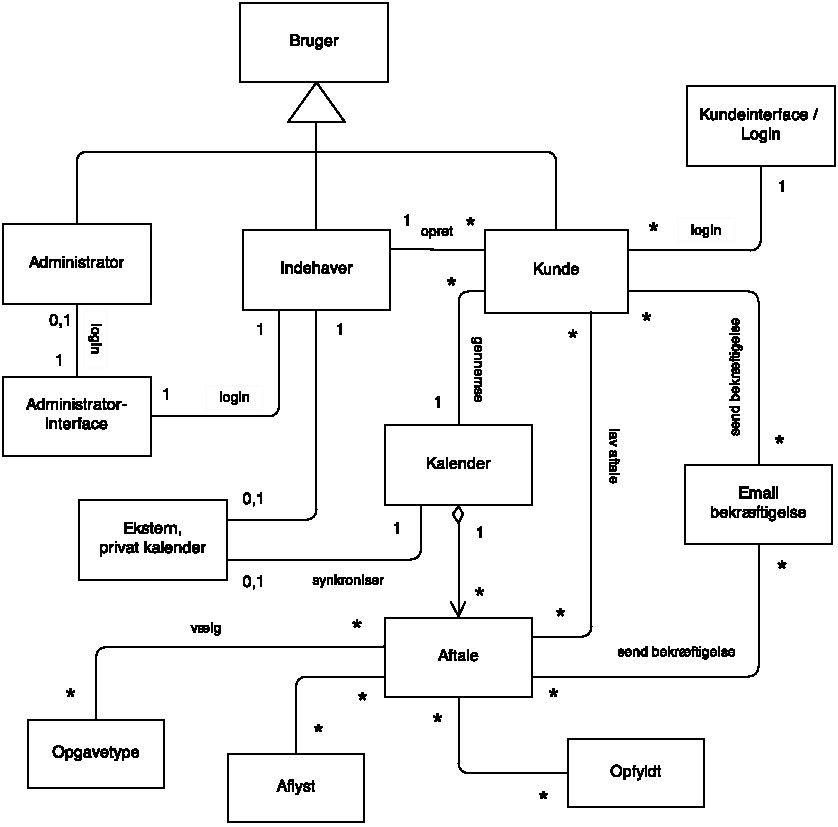
\includegraphics[width=12cm, height=12cm]{problemomr.pdf}
\caption{UML-diagram over problemområdet}
\label{fig:problem}
\end{center}
\end{figure}

Her følger en liste af de klasser, vi har identificeret i problemområdet:

\begin{itemize}
\item Bruger: Kunde, administrator, indehaver. Går igen fra
	anvendelsesområdet.
\item Tre interfaces. Et til kunderne, et til systemadministratoren og et til
	KT's indehaver til daglig brug.
\item Et kundekartotek, hvor KT's indehaver løbende kan tilføje kunder.
\item Kalenderen, som kunderne kan bruge, når de skal finde en ledig tid, og
	som KT's indehaver kan bruge i sit daglige, travle arbejde.
\item Aftale. Kunderne booker en aftale i kalenderen.
\item En aftale kan både være aflyst og opfyldt, hvis den ikke længere er
	aktuel.
\item Da KT har både mundtlige, skriftlige og andre opgaver, skal kunden
	oplyse typen på arbejdet.
\item Når kunden har booket en aftale, sendes der en bekræftende email tilbage
	til kunden med det aftalte tidpunkt, og KT's indehaver får ligeledes
	en email med dato, klokkeslet og opgavetype.  
\item KT's indehaver har et ønske om at kunne synkronisere hendes eksterne,
	private kalender med vores it-løsning.
\end{itemize}

Vi begynder denne gennemgang af problemområdet med de tre interfaces, hvor
brugerne først møder systemet. Systemadministratoren får sit eget selvstændige
interface, idet vedkommende skal kunne tilgå systemet med samtlige
rettigheder. Som vi også nævnte under gennemgangen af anvendelsesområdet, så
skal KT's indehaver alene i kraft af, at hun er eneste medarbejder, også have
adgang til systemet gennem administratorinterfacet, så hun f.eks. kan
tilføje nye kunder til kundekartoteket. Derudover får KT sit eget interface
til daglig brug, så Souzane kan gennemgå kalenderen uden at være nervøs for at
ødelægge aftaler eller data. KT's kunder vil også blive præsenteret
for et login interface, når de navigerer til hjemmesiden. Efter login vil der 
være adgang til kalender og bookingsystemet. Det skal være muligt at vise dage, 
uger og måneder, og brugere skal kunne søge i kalenderen udfra de samme
kriterier.\\
Det er også et krav til kalenderen, at kunden let kan skelne mellem ledige
tidspunkter og allerede bookede aftaler ved hjælp af et farvesystem. Her vil
ledige tidspunkter være markeret med grøn skrift og aftaler med rød skrift. \\
Dette fører modelleringen af problemområdet videre til aftaleklassen. Der vil 
være en naturlig sammenhæng mellem kalender og aftale, og derfor er de
sammenkoblet ved aggregering. En kunde kan lave en eller flere aftaler på
samme tid, og vedkommende vil efter hver indgået aftale automatisk modtage en 
bekræftende email med dato og tidspunkt. Dette ses til højre i UML-diagrammet,
hvor emailen autogenereres og sendes tilbage til kunden. Vi har suppleret aftale
klassen med to tilhørende klasser: aflyst og opfyldt, som er de to tilstande,
en aftale kan være i. (En igangværende aftale har vi ikke fundet vigtig nok
til at modellere).\\
Der skal i kalenderen være mulighed for at aflyse en
allerede indgået aftale, og proceduren vil være den samme som ved oprettelsen.
Kunden logger på, aflyser aftalen og modtager en autogenereret email som
bekræftigelse. Hvorvidt KT er interesseret i at beholde gamle og udløbne aftaler 
i kalenderen, står endnu ikke helt klart. De kunne bibeholdes som en form for
kalenderhistorie eller logbog, hvis KT skal gennemgå gamle aftaler i
forbindelse med fakturering eller anden opgørelse, men det ville være mest
hensigtsmæssigt at sætte en grænse, så databasen ikke fyldes op med gamle,
ligegyldige aftaler.\\ 
Det sidste, vi vil berøre i problemområdet, er det usikre punkt om samspillet
mellem en ekstern kalender og vores eget kodede kalendersystem. KT's indehaver
har sin egen private Google kalender, som hun gerne vil synkronisere med vores
it-løsning for at overføre hendes private aftaler, så alt er samlet i èn
kalender. Kompleksiteten i denne opgave er måske for stor, så måske må
vi stille K. Translation i udsigt, at private aftaler skal indtastes manuelt i
kalenderen, men det må vi tage stilling til, når kernefunktionerne er
implementerede. \\
Hermed slutter vi gennemgangen af anvendelses- og problemområdet. Den
ovenstående modellering vil ligge til grund for det videre design og endelige
system. 

\pagebreak

\section{Use-cases}
I dette afsnit vil vi beskrive og analysere de vigtigste funktionelle
egenskaber ved systemet. Udgangspunktet er kravindsamlingen, som her udvikles
til en high-level use case model, hvori vi efterfølgende identificerer de tre
vigtigste use cases. Vi har samlet alle use cases og præsenterer dem i det
medfølgende højniveau-diagram. Se figur \ref{fig:use}.

\begin{figure}[!ht]
\begin{center}
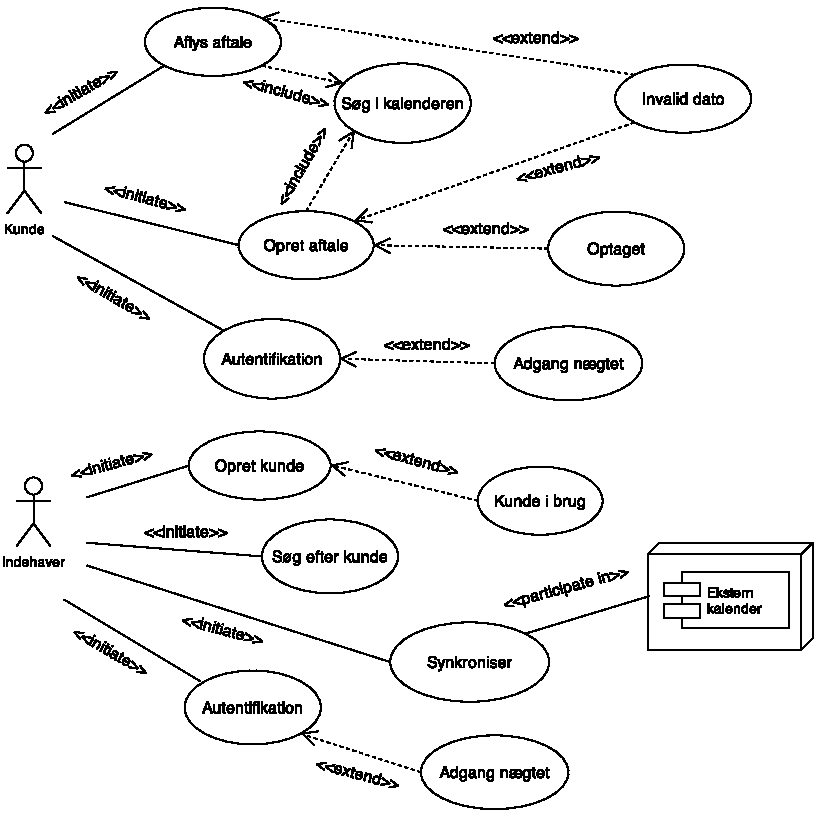
\includegraphics[width=12cm, height=12cm]{highlevel.pdf}
\caption{Højniveau-diagram bestående af samtlige identificerede use cases.}
\label{fig:use}
\end{center}
\end{figure}

De enkelte use cases er udviklede fra de funktionelle krav, og konteksten er
problemområdet, der vækkes til live i use case handlingsforløbene. 
Aktørerne i højniveau-diagrammet er alle hentede fra anvendelseområdet.
Indehaveren af KT er i dette scenario også systemadministrator, idet hun selv vil
skulle udfylde denne rolle på længere sigt, og derfor er denne aktør ikke
medtaget som en selvstændig klasse. Vi mener heller ikke, at det vil tilføje
modellen mere værdi også at modellere systemadministratoren, da vedkommendes
use cases i så fald vil være et subsæt af indehaverens.\\
Hvis to use cases indeholder det samme begrænsede handlingsforløb, har vi modelleret
dette med et ``include'' forhold. F.eks. kan en potientel kunde søge i kalenderen,
både når vedkommende opretter en aftale og når vedkommende aflyser en aftale. Dette
er med til at nedsætte kompleksiteteten i use case modellen og fjerne
redundans. Det samme gør sig gældende med ``extend'' forholdene, der
modellerer undtagelser og fejltilstande som f.eks. systemets reaktion på
ulovlige datoer eller mislykket login.\\
Vi har valgt de fire vigtigste use cases ud og præsenterer dem her med 
sekvensdiagrammer. Første use case ``Opret kunde'' kan ses i tabel 3.\\

\begin{tabular}{l p{10cm}}
Use case navn & Opret kunde \\ \hline
Deltagere & \nextitem Initieret af KT's indehaver
            \nextitem Kommunikerer med kunde \\ \hline
Handlingsforløb &
	\nextitem Indehaveren af KT logger på systemet som administrator. 
	\nextitem Administratorinterfacet viser menuen.
	\nextitem Indehaveren navigerer til menupunktet, hvor man kan tilføje nye
		kunder.
		\nextitem Interfacet præsenterer en formular til indehaveren
	\nextitem KT's indehaver udfylder samtlige formularfelter med
		kundens stamdata og anden kontaktinformation. Derefter
		sender hun formularen.		
	\nextitem Administratorinterfacet tilføjer kunden til kundekartoteket
	og autogenererer en email, der sendes til den aktuelle kunde
		med besked om, at vedkommende nu kan logge på systemet for at
		booke en tid.
	\nextitem KT's indehaver logger af systemet. 
	\nextitem Interfacet lukkes.
	\\ \hline
	Indgangs betingelse &
		\nextitem KT's indehaver er logget på administratorinterfacet. 
		\nextitem Pågældende kunde er ikke oprettet i kundekartoteket. 
		\\ \hline
Exit betingelse & 
	\nextitem Pågældende kunde er nu tilføjet til
			kundekartoteket.
		\nextitem Der ligger en bekræftende email i den pågældende kundes
			indbakke.
		\nextitem KT's indehaver er logget af systemet.\\ \hline
\end{tabular}
\begin{center}
\textbf{Tabel 3} Opret kunde use case.
\end{center}
\vspace{0.5cm}

Denne use case beskriver, hvordan K. Translations indehaver opretter en ny
kunde i kundedatabasen. I vores gennemgang vil vi fokusere på at identificere
``entity'', ``boundary'' og ``control'' objekterne i use casen. Dette kan 
ses som en forløber for vores valg af ``Model-View-Controller'' 
arkitekturen og Django frameworket, som det fremgår af afsnittet omhandlende 
softwarearkitektur, eftersom ``Model'' kan kortlægges til ``entity'', ``view''
til ``boundary'' og ``controller'' til ``control''. I det efterfølgende vil vi dog 
bruge de danske betegnelser, som er henholdsvis entitet, grænseflade og kontrol. \\
De to aktører i use casen er KT's indehaver og en kunde. Indehaveren
igangsætter use casen og er den aktive part, mens kunden kun medvirker
passivt. Grænsefladeobjekterne i use casen er administratorinterfacet, hvor indehaveren
logger på systemet, og formularen, hvor hun indtaster kundens stamdata. Den
bekræftende email er også en del af grænsefladen, selvom den ikke går til 
indehaveren men til kunden. Kundekartoteket er den ene entitet i use casen og
kunde den anden. Her tænker vi ikke på kunden som aktør men som en entitet,
der oprettes undervejs udfra de indtastede stamdata. Det er umiddelbart
lettere at identificere kontrollen i det medfølgende sekvensdiagram, så vi
henviser til figur \ref{fig:opret}. Her fremgår det, at systemet har en
administratorkontrol, der er ansvarlig for at oprette entiteten: Kunde og
grænsefladerne: Email samt Aftaleformular. Dette er måske snarere en for tidlig
truffet design beslutning, som ikke fremgår af use casen, men krontrol objekter
skabes ofte af grænseflader, der kan tilgås af aktøren for at igangsætte 
handlingsforløbet.    

\begin{figure}[!ht]
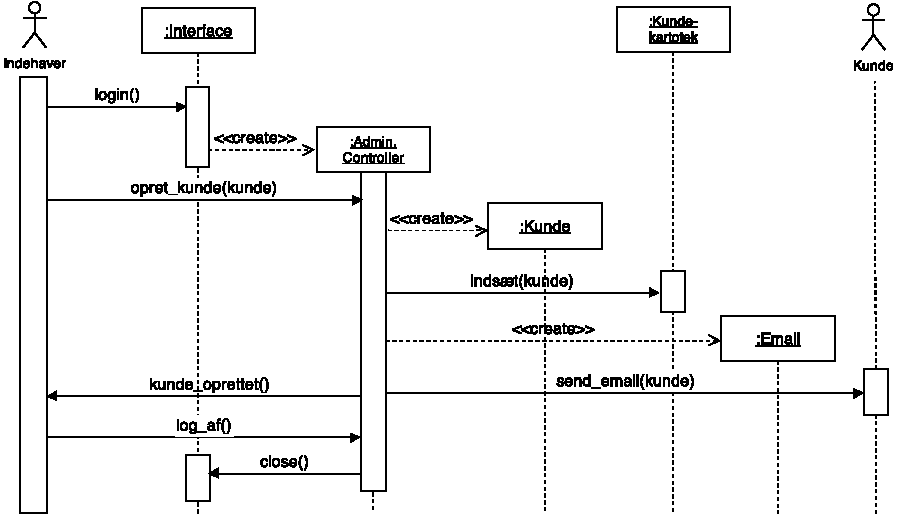
\includegraphics[width=14cm, height=10cm]{seqtwo.pdf}
\caption{Sekvensdiagram for Opret kunde use case.}
\label{fig:opret}
\end{figure}

Den anden use case, vi har valgt, hedder ``Opret aftale''. Se tabel 4.  Her 
logger en kunde på systemet for at booke en aftale med tolkeservicen, og
vedkommende skal både oplyse dato, klokkeslet og opgavetype. Igen er der to
aktører: kunden og KT's ejer. Men rollerne er byttede om i forhold til den
første use case. Nu er kunden den aktive part, og KT's ejer er den passive,
idet hun kun deltager i use casen for at modtage en email.\\


\begin{tabular}{l p{10cm}}
Use case navn & Opret aftale \\ \hline
Deltagere & \nextitem Initieret af KT's kunde
            \nextitem Kommunikerer med Indehaveren af KT\\ \hline
Handlingsforløb &
	\nextitem KT's kunde navigerer til KT's hjemmeside, hvor kunden logger
	på med det personlige password.
	\nextitem Kalenderkontrollen henter kalenderen og viser den til
	kunden.
	\nextitem Kunden vælger at oprette en aftale.
	\nextitem Kalenderkontrollen henter en formular, som kunden skal
	udfylde.
	\nextitem Kunden indtaster datoen og klokkeslettet for den ønskede 
	aftale og bekræfter.
	\nextitem Kontrollen validerer dato samt klokkeslet og præsenterer
	kunden for en menu med forskellige aftaletyper.
	\nextitem Kunden vælger den ønskede aftaletype og bekræfter.
	\nextitem Kontrollen opretter aftalen i kalenderen og sender
	automatisk en email til både kunden og indehaveren af KT. 
	\nextitem Kunden logger af kalenderen.
	\\ \hline
	Indgangs betingelse &
		\nextitem KT's kunde er logget på kalenderen. 
		\nextitem Kalenderen indeholder ingen aftaler på det af kunden
		ønskede tidspunkt.
		\\ \hline
Exit betingelse & 
	\nextitem Der er oprettet en aftale i kalenderen på det ønskede
	tidspunkt. 
		\nextitem Der ligger en bekræftende email i den pågældende kundes
			indbakke.
		\nextitem Det ligger en email i KT's indehavers
			indbakke med dato og tidspunkt for aftalen. 
		\nextitem Kunden er logget af systemet.\\ \hline
		Kvalitets krav & Da det er muligt for kunden at søge i
		kalenderen, kan denne use case på et vilkårligt tidspunkt
		inkludere use casen  ``Søg i kalender''. Hvis dette sker, kan
		kunden søge i kalenderen, enten ved at bladre frem èn dag eller uge
		ad gangen eller ved at søge på en dato længere ude i
		fremtiden.\\ \hline
\end{tabular}
\begin{center}
\textbf{Tabel 4} ``Opret aftale'' use case.
\end{center}
\vspace{0.5cm}


Grænsefladeobjekterne er KT's hjemmeside, som use casen indledes fra, og
formularerne, der udfyldes af kunden undervejs. Den bekræftende email er
ligeledes en del af grænsefladen. Kalenderen og aftalen er entiteter, og som
det fremgår af det medfølgende sekvensdiagram, så udgøres kontrolobjektet af en
``kalender controller''. Se figur \ref{fig:aft}. 
Igen består første kolonne af den initierende aktør, anden kolonne er
grænsefladen, som aktøren bruger til at igangsætte use casen, og tredie
kolonne indeholder kontrol objektet, som undervejs når at oprette to
grænsefladeobjekter mere samt endnu en entitet.

\begin{figure}[!ht]
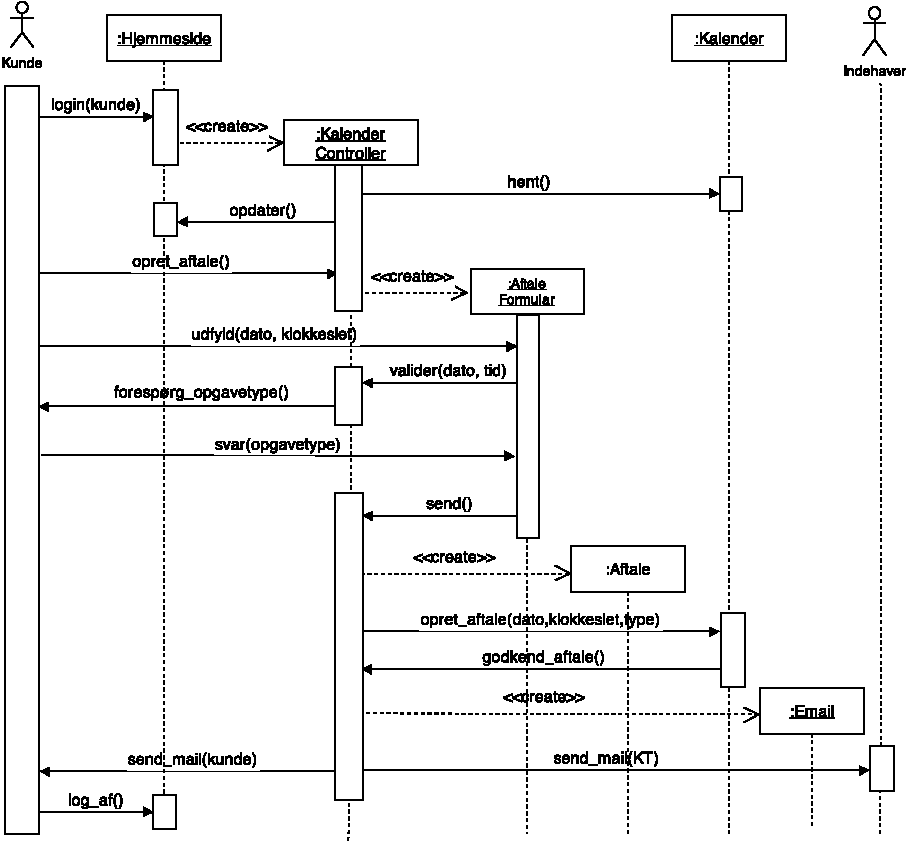
\includegraphics[width=14cm, height=11cm]{seq.pdf}
\caption{Sekvensdiagram for ``Opret aftale'' use case.}
\label{fig:aft}
\end{figure}

Efter at have vist to almindelige use cases, har vi til sidst valgt, 
at fokusere på de extraordinære forhold, der gør sig gældende ved ``extend''
use cases. Derfor viser vi to små use cases: ``Optaget'' og ``Ulovlig
dato'', men vi gennemgår kun selve undtagelserne, eftersom konteksten for
disse use cases er ``Opret aftale'' use casen fra tabel
1 og figur \ref{fig:aft}. Handlingsforløbene før og efter undtagelserne træder i
kraft vil være præcise gentagelser af ``Opret aftale'' use casen; man skal
altså forestille sig denne use case på et givent tidspunkt i forløbet
blive udvidet med en af de følgende to use cases. Se tabel 5 og 6.\\ 



\begin{tabular}{l p{10cm}}
Use case navn & Optaget \\ \hline
Deltagere & \nextitem Kommunikerer med KT's kunde. 
            \\ \hline
Handlingsforløb &
	\nextitem Kunden oplyser typen på opgaven og bekræfter. 
	\nextitem Kalenderkontrollen prøver at oprette en aftale i kalenderen
	på det givne tidspunkt, men bliver nægtet adgang, fordi der allerede
	ligger en aftale på dette tidspunkt. Kontrollen beder kunden om at
	finde en ny tid.
	\nextitem Kunden indtaster et nyt tidspunkt i formularen og bekræfter. 
	\nextitem Formularen validerer tidspunktet.
	\\ \hline
	Indgangs betingelse &
		\nextitem Denne use case udvider ``Opret aftale'' use casen.
		Den initieres, når kontrollen prøver at indsætte en aftale i
		kalenderen på et tidspunkt, hvor der i forvejen eksisterer en
		aftale. 
		\\ \hline
Exit betingelse & \dots
	\\ \hline
\end{tabular}
\begin{center}
\textbf{Tabel 5} ``Extend'' use case: ``Optaget''.       
\end{center}
\vspace{0.5cm}


\begin{tabular}{l p{10cm}}
Use case navn & Ulovlig dato \\ \hline
Deltagere & \nextitem Kommunikerer med KT's kunde.
            \\ \hline
Handlingsforløb &
	\nextitem Kunden oplyser kontrollen om, at vedkommende vil oprette en
	aftale.
	\nextitem Kontrollen opretter en formular til aftalen.
	\nextitem Kunden indtaster dato og klokkeslet for aftalen og
	bekræfter.
	\nextitem Formularen prøver at validere tidspunktet, men den fejler.
	Kontrollen beder kunden indtaste et nyt tidspunkt.
	\nextitem Kunden indtaster dato og klokkeslet for den nye aftale og
	bekræfter.
	\nextitem Formularen prøver at validere tidspunktet og godkender.
	Kontrollen spørger kunden om opgavetypen.
	\nextitem Kunden oplyser opgavetypen og bekræfter.
	\\ \hline
	Indgangs betingelse &
		\nextitem Denne use case udvider ``Opret aftale'' samt ``Aflys
		aftale'' use cases. Den initieres, når formularen ikke kan
		validere tidspunktet for kundens aftale, fordi kunden har
		indtastet et ikke eksisterende tidspunkt.  
		\\ \hline
Exit betingelse & \dots
	\\ \hline
\end{tabular}
\begin{center}
\textbf{Tabel 6} ``Extend'' use case: ``Ulovlig dato''.       
\end{center}
\vspace{0.5cm}

Grænseflade-, kontrol- og entitetobjekterne i de to ``extend'' use cases vil
være magen til objekterne i de oprindelige use cases, der udvides med disse
undtagelser, som det også fremgår af de medfølgende sekvensdiagrammer. Se figur
\ref{fig:extseq} for begge sekvensdiagrammer. \\

\begin{figure}[!ht]
	\begin{center}
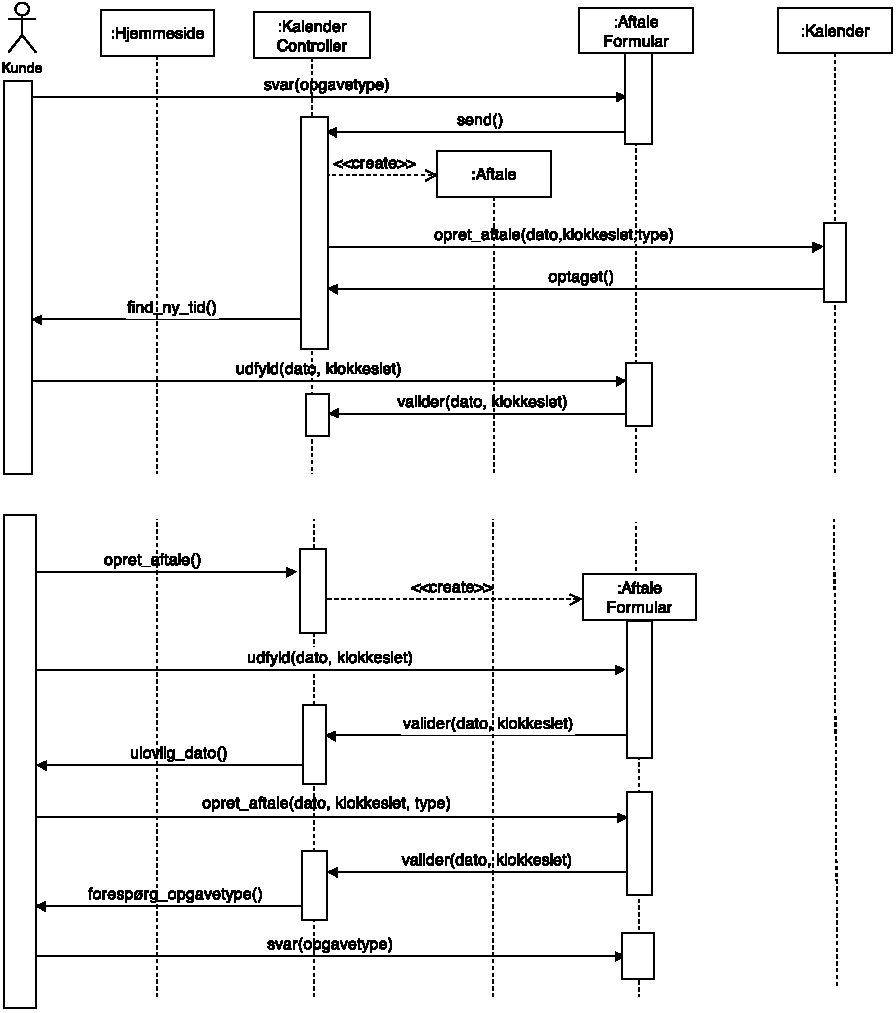
\includegraphics[width=13cm, height=15cm]{ext.pdf}
\caption{Sekvensdiagram for ``Optaget'' samt  ``Ulovlig dato''.}
\label{fig:extseq}
\end{center}
\end{figure}

Vores arbejde med disse use cases og sekvensdiagrammer har betydet, at vi har
været tvunget til at se systemet fra brugerens synsvinkel, og at vi har
overvejet flere desingrelaterede problemstillinger. F.eks har identifikationen 
af entitet-, grænseflade- og kontrolobjekterne betydet, at vi har lagt os fast
på en systemarkitektur, ``Model-View-Controller'', samt et framework i det
MVC-baserede Django. Det vil yderligere hjælpe os, når vi i netop Django skal
til at definere vores modeller, templates og viewfunktioner, at vi har bestemt
og afgrænset objekternes opførsel, så de hurtigt kan sættes ind i en MVC
kontekst. Derudover har vi med ``extend'' use cases set, hvorhenne i systemet
undtagelser og exceptionel opførsel kan blive et problem, der skal håndteres. 


\section{Softwarearkitektur}
Det kan være en stor udfordring, at finde den rigtige softwarearkitektur i et
systemudviklingsprojekt. Vi har selv overvejet flere forskellige arkitekturer 
og vil i dette afsnit argumentere for vores valg og fravalg. Først overvejede
vi en multilagdelt arkitektur i form af 3-tier arkitekturen. Her kunne vi i
datalaget gemme de oprettede brugere og bookede aftaler i en database.
Forretningslogikken kunne placeres i mellemlaget og kodes med PHP.
Brugerinterfacet ville ligge i præsentationslaget og tilgås gennem brugerens
browser. Vi fravalgte dog denne løsning af flere grunde. Vi fandt det ikke
strengt nødvendigt med tre lag, da det tredie lag ikke ville betyde
nævneværdige forbedringer i forhold til en almindelig client-server model.
Derudover kunne vi også uforvarent komme til at introducere flere
sikkerhedsbrister, hvis vi havde kodet mellemlaget i PHP, da dette kræver, at 
man er ekstrem opmærksom på validering af brugerinput. Én maliciøs SQL-injection
kan slette en hel database og alle aftaler, hvilket ville være katastrofalt for
KT. Da vores kalendersystem ikke kræver andet for at fungere end en bruger med
en browser, der kan logge på KT's server, besluttede vi derfor, at holde 
arkitekturen så overskuelig som mulig ved at bruge client-server modellen. \\
Dernæst valgte vi det Model-View-Controller (MVC) baserede web framework Django til
at understøtte client-server arkitekturen. Se figur \ref{fig:mvc}.\\

\begin{figure}[!ht]
	\centering
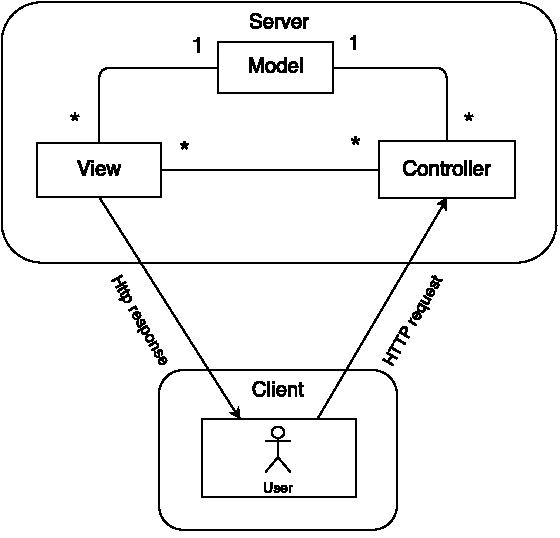
\includegraphics[width=10.5cm, height=9.5cm]{mvc.pdf}
\caption{Model-View-Controller arkitektur superimposeret på client-server.}
\label{fig:mvc}
\end{figure}

Django kommer med et enkelt og praktisk administratorinterface, der kan blive
særdeles nyttigt for os under systemudviklingen og for indehaveren af KT på
længere sigt. Desuden får vi mulighed for at benytte Django's mange indbyggede 
applikationer. Vi kommer til at bruge moduler, der understøtter implementering af
html formularer, og som også er i stand til at validere brugerinput i disse,
og moduler for brugeroprettelse og autentifikation. Det betyder for os, at der er
færre muligheder for at introducere fejl og sikkerhedsmangler til
systemet. En af Djangos helt store styrker, som udspringer af MVC arkitekturen,
er den løse kobling og strenge adskillelse mellem de forskellige dele af modellen.
Det betyder, at vi let kan ændre, slette eller tilføje i eksisterende dele uden at
bekymre os om afhængigheder mellem delene. \\
Fordi views i Django terminologi består af templates, og controllers består af
viewfunktioner, er det måske mere rigtigt at kalde Django for en Model-View-Templates
(MTV) arkitektur, men vi bibeholder den normale konvention og skriver MVC. Vores
model kommer til at bestå af de aftaler, som KT's kunder booker ind i kalenderen.
D.v.s at domænerne i den bagvedliggende database, som modellen kortlægges til og 
fra, udgøres af datoen og klokkeslettet for aftalen, opgavetypen samt navnet
på kunden. Django's templates står som sagt for præsentationen, og vi
påtænker at bruge en basisskabelon til hjemmesiden, der kan udvides med
tilpassede templates, når logikken kræver det. Selve forretningslogikken bliver 
implementeret i Django's viewfunktioner. (Controller i MVC). Det er bindeleddet
mellem modellen og præsentationen, og det er her kernefunktionaliteten kommer til at 
sidde. Eftersom Django i virkeligheden er en samling Python biblioteker, vil vi kode 
systemet i programmeringssproget Python. Det er også et godt valg, fordi det ene
medlem i vores tomandsgruppe har erfaring med Python, og det andet medlem ikke har.
Python kan læres relativt hurtigt, så det ene medlem får muligheden for at
lære det undervejs i projektet, mens det andet medlem kan lære det fra sig
evt. gennem pair-programming. \\ 


\section{Projektplan}
Adskillige forelæsninger i Systemudviklingskurset har handlet om agil
projektledelse og systemudvikling. Vi har fundet en sådan iterativ og
inkremental tilgang til projektet spændende og kunne derfor godt tænke os at
systemudvikle inden for rammerne af de agile principper, som vi bl.a. har
stiftet bekendsskab med i artiklen ``Jeff Sutherland's Scrum
Handbook''\cite{scrum}. Det vil dog ikke være muligt, at gennemføre projektet
i komplet overensstemmelse med Scrum og alle de agile regler. For det første
vil det betyde, at vores kunde skal afse betydelig mere tid til projektet,
end hun umiddelbart har planlagt, hvis hun løbende skal opdate ``Product
Backlog'' og deltage i prioriteringsmøder ved hver sprints begyndelse.
Derudover vil det ikke være realistisk, at vi selv holder daglige Scrum møder,
og at vi kan levere al den dokumentation et virkeligt Scrum forløb
forudsætter som f.eks. de daglige overslag over vores egne fremskridt i forhold
til opgaverne i den aktuelle sprint. Derfor vil vi slække på nogle af 
reglerne, og vi håber at kunne gøre det uden at bevæge os alt for langt væk fra 
den virkelige agile Scrum systemudvikling.\\
I stedet for de daglige estimeringer over projektets fremadskriden, har vi
valgt at nøjes med et overordnet burndown diagram for hele projektet. Se figur
\ref{fig:bd}. (Et brundown diagram for en enkelt sprint vil være magen til,
men værdierne på førsteaksen vil være dage i stedet for uger, og værdierne på
andenaksen vil være mindre). 

\begin{figure}[!ht]
	\centering
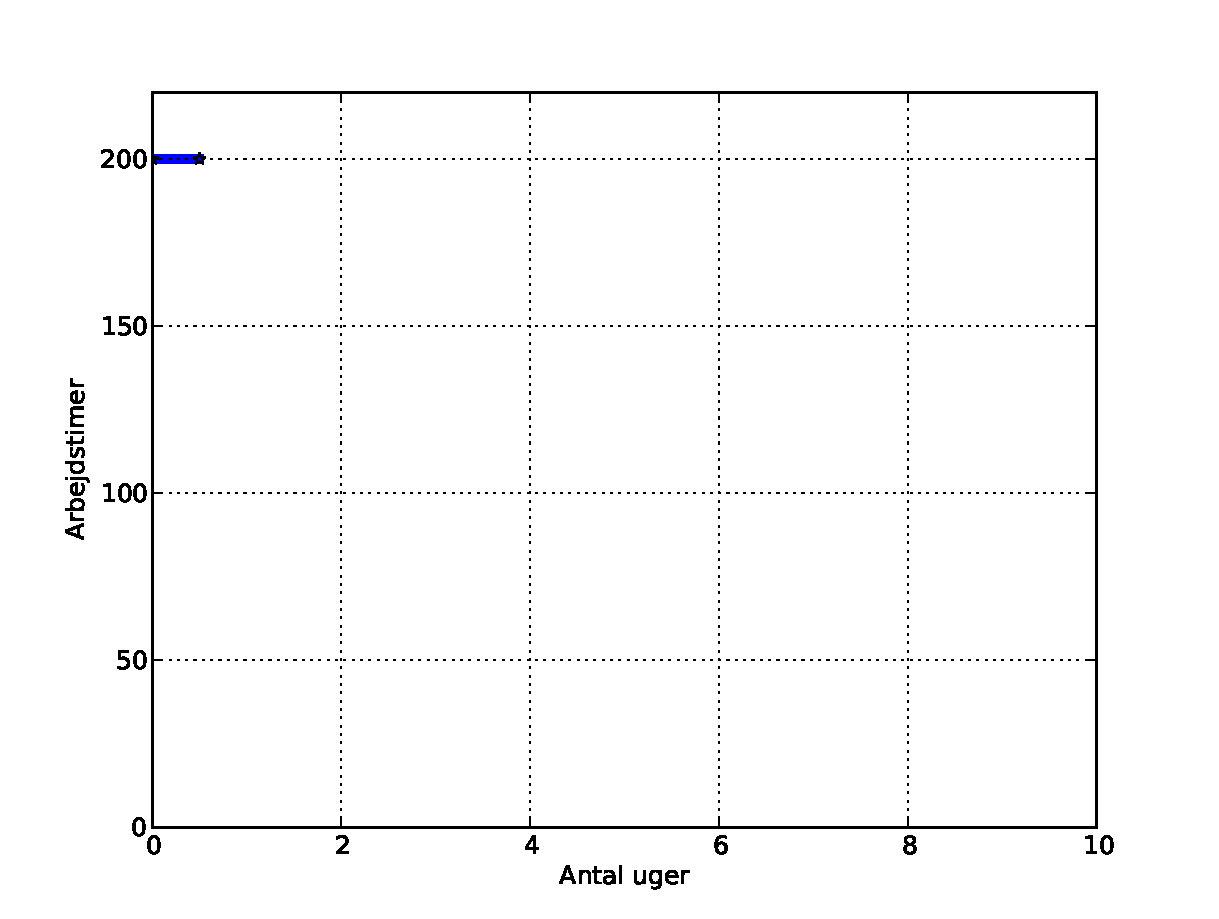
\includegraphics[width=13cm, height=9cm]{burndown.pdf}
\caption{Burndown diagram over projektforløbet}
\label{fig:bd}
\end{figure}

Vi har som udgangspunkt afsat mellem 8 og 10 uger til det agile projektforløb
og bedømt den påkrævede arbejdsindsats til at være 200 timer, hvilket vil sige 100
timer til hver, da vi er to mand i gruppen. Dette overslag er dog yderst
usikkert, men vi har aldrig prøvet at arbejde på denne måde før, så det bliver
spændende at se, om vores estimationer bliver mere præcise undervejs. Vi har
planlagt at udvikle i sprints af 14 dages varighed, men vi kan udvide dette til 3
uger, hvis et af punkterne i produkt backloggen forekommer mere omfangsrigt.\\
Indehaveren af K. Translation har ofte meget travlt og kan som sagt ikke
deltage i hvert nyt sprintmøde. Derfor har vi besluttet at simulere disse
møder ved, at vi selv skriver og opdater produkt backloggen og gør det med
udgangspunkt i kravspecifikationen. Vi bliver herved in effect vores egen 
proxykunde ! Den indledende produkt backlog kan ses i tabel 1.

\begin{center}
	\begin{tabular}{|p{8cm}|l|l|l|}
		\hline
Punkt & Prioritet & Værdi & Indsats \\ \hline
Som bruger af KT's hjemmeside bliver man præsenteret for en kalender, hvori man
kan booke en aftale med KT. & 1 & Høj &  50 \\ \hline
Som KT's kunde møder man et login interface, når man navigerer til hjemmesiden. & 2 &
Høj & 15  \\ \hline
KT skal have muligheden for løbende at tilføje kunder til databasen. & 3 & Høj
& 15 \\ \hline
Man skal som kunde modtage en bekræftende email efter at have lavet en aftale
i kalenderen. KT skal ligeledes modtage en email med aftalen. & 4 & Middel & 10  \\ \hline
Som kunde bliver man præsenteret for en lille menu, hvor man skal vælge typen
på arbejdet. & 5 & Lav & 20\\ \hline
Som kunde skal man kunne søge i kalenderen ved hjælp af dato eller klokkeslet.
& 6  & Middel &  25 \\ \hline
Indehaveren af KT vil gerne kunne synkronisere sin eksterne kalender med
hjemmesidens kalender og på den måde overføre sine private aftale. & 7 & Lav &
 35 \\ \hline
KT ønsker en hjemmeside med kontaktinformation, billeder og et enkelt design.
& 8 & Middel & 12 \\ \hline
\end{tabular}
\end{center}
\begin{center}\textbf{Tabel 1} Produkt Backlog
\end{center}
\vspace{0.5cm}

KT's ønsker står i prioriteret rækkefølge, og vi har yderligere tilføjet en
kolonne, hvor vi kan estimere nytteværdien af punktet med Høj, Lav eller
Middel. Sidste kolonne viser vores bedømmelse som udviklere af den påkrævede
arbejdsindsats. Ofte vil punkterne i produkt backloggen være formuleret som
små brugerhistorier eller endda som deciderede use cases. Dernæst har vi
valgt ud, hvilke punkter vi koncentrerer os om i den første sprint. Dette
fremgår af tabel 2, som er Sprint Backloggen. Punkterne bliver yderligere
delt op i sprint opgaver, og hver udvikler påtager sig et antal opgaver og
kommer igen med en bedømmelse af den påkrævede arbejdsindsats i timer. Sprint
backloggen bliver dermed udgangspuktet for systemudviklingen i den
efterfølgende sprint. 


\begin{center}
	\begin{tabular}{|l|p{4cm}|l|l|}
		\hline
		Backlog punkt & Sprint opgave & Frivillig & Indsats\\ \hline
		\multirow{4}{4cm}{Som KT's kunde møder man et login interface,
		når man navigerer til hjemmesiden.} & Oprette en Django
		applikation & Omar  & 2 \\
		& Skriv login interfacet & Morten & 6 \\
		& Test login interfacet & Omar & 3 \\
		& Integrer interfacet med resten af hjemmesiden & Morten og Omar
		& 4 \\ \hline
		\multirow{3}{4cm}{KT ønsker en hjemmeside med
		kontaktinformation, billeder og et enkelt design.} &
		Skrive basisskabelonen til Django & Morten & 5 \\
		& Udvid basisskabelonen med Djangos ``extend''-skabeloner & Morten & 5
		\\ & Test hjemmesiden i flere forskellige browsere & Omar & 2 \\
		\hline

	\end{tabular}
\end{center}

\begin{center}
\textbf{Tabel 2} Sprint Backlog
\end{center}

\vspace{0.5cm}



\section{Designing for usability: key principles and what designers think}
Artiklen \emph{Designing for usability: key principles and what designers
think} \cite{usa} skrevet af Gould og Lewis handler om systemdesign set fra et
brugervenligt perspektiv. Forfatterne begynder artiklen med at anbefale tre
desingprincipper: tidlig fokus på brugere, empirisk analyse og iterativt
design. De påpeger også løbende i artiklen det store spænd, der er mellem,
hvad systemudviklere og programmører siger, og hvad de rent faktisk gør, for
selvom de alle kan tilslutte sig de tre designprincipper, og selvom de alle
mener, at de overholder dem i deres egne projekter, viser forfatternes
forskning, at dette ikke er tilfældet, som det også fremgår af tabel 1 i
artiklen. \\
Dernæst kommer Gould og Lewis selv med en række bud på, hvorfor deres ellers
oplagte principper ikke bliver fulgt i virkeligheden: at de ikke er værd at
følge, at de bliver forvekslet med lignende men afgørende forskellige ideer,
at værdien af brugerinteraktion er vurderet forkert, at de er upraktiske. Det
viser, at principperne slet ikke er oplagte alligevel i virkelige
systemudviklingsforløb, og at der er mange mentale samt praktiske
forhindringer, hvis de skal føres ud i livet. \\
Forfatterne uddyber de tre principper ved at dele et projekt op i en
indlendende designfase og en iterativ udviklingsfase. Specielt er der i den
indledende fase fokus på brugerne, på test af interfaces og på at opstille
målbare adfærdsmæssige målsætninger. I den iterative udviklingsfase er fokus
på fleksible prototyper og modulær implementering, hvilket indebærer, at
brugertests kan fortsætte så langt ind i udviklingen som muligt. Forfatterne
afslutter artiklen med en konkret case study: et audio distribueringssystem
fra IBM, der mest af alt minder om en mellemting mellem en sms, en email og en
diktafon, hvor de tre desingprincipper med succes blev fulgt. 
Artiklen fokuserer meget på at forstå brugerne i anvendelsesområdet, som også
OOSE bogen og OOAD kapitlerne gør meget ud af. Vi synes dog, at artiklen går
et skridt videre ved at kvantificere adfærdsmæssige aspekter og kræve
empirisk, målbare beviser for brugertests. Ellers kan mange af forfatternes
forslag genkendes fra andre af vores pensums artikler.  Rolf Molich skriver i
``User Testing, Discount User Testing'' om Thinking-aloud processen: ``It can
be used to user test early paper prototypes of a new application for
conceptual clarity, and it can be used to test late beta version of a new
application interface for disasters.'' Dette er fint i tråd med Gould og
Lewis, og Molich henviser da også til artiklen i litteraturfortegnelsen. \\
Artiklens fokus på fleksible prototyper kan også genkendes fra Ehn og Kyng
artiklen: ``Mocking it up''. Begge artikler fremhæver vigtigheden af at kunne
simulere brugerinterfacet på den ene eller anden måde. Det kan være så
simpelt som tegninger af skærmen, menuerne eller interfacet, eller det kan
være mere avanceret, hvor der er mulighed for at reagere realtime på brugerens
input. Begge artikler indeholder også virkelige case studies, hvor mock-ups
indgik som en integreret del af designfasen, og hvor dette resulterede i
ændringer i produkterne: IBM's audio-distribuerings system og et computerstyret
pakke sorteringssystem fra sverige.\\
Forfatterne lægger også vægt på det iterative projektforløb, som muliggører
radikale ændringer selv langt inde i et udviklingsforløb evt. på grund af ny
brugerforståelse. Dette er selve grundstenen i den agile systemudvikling, som
vi kender det fra Jeff Suterland's ``Scrum Handbook'' og i mindre grad  fra
Jim Highsmiths ``Extreme Programming''. \\
Vi synes, at de to obligatoriske artikler udgører et sjovt match. I den ene 
artikel hævder forfatterne, at de har fundet systemudviklingens tre vise sten.
(Gould og Lewis' tre principper). I den anden artikel hævder forfatterne, at disse
vise sten slet ikke eksisterer, hvorfor man må ``snyde sig til dem''.  

\section{A rational design proces: How and why to fake it}
Den anden artikel \emph{A rational design proces: How and why to fake it} af
David Parnas og Paul Clements argumenterer for, hvorfor software designprocessen
altid vil være en tilnærmelse til det ideelle systemudviklingsforløb. Forfatterne
begynder med at opliste, hvorfor er projektforløb ikke kan foregå fuldstændig
rationelt. Den vigtigste forhindring skal igen findes i brugerne af systemet. Som
i den foregående artikel frmehæves det, hvorledes brugerne ikke altid ved, hvad
de virkeligt vil have, og at dette kan føre til ændringer langt inde i
designprocessen. Det betyder, at designere er nødt til at ``backtracke'',
hvilket invaliderer det oprindelige, rationelle beslutningsforløb. En anden
forhindring er designernes forudfattede ideer, som kan føre til, at ideer,
software samt designmønstre fra tidligere projekter ønskes genbrugt, måske af
økonomiske eller tidsmæssige hensyn, selvom de ikke passer til det pågældende
projekt. \\
Selvom forfatterne hævder, at det ideelle projektforløb ikke eksisterer,
argumenterer de for, hvorfor designere skal ``fake'' det, og her er
dokumentation alfa-omega. Dokumentationen af et projekt starter allerede med
kravspecifikationen, som er et udgangspunkt, programmører altid kan gå tilbage
til for at danne sig et overblik over systemets opførsel. Derudover skal hele
modulstrukturen dokumenteres undervejs i projektet, og det samme skal modulernes 
interfaces. Alle designbeslutninger skal noteres, valg og fravalg,
alternativer og rationalerne bagved beslutningerne beskrives. Dette har vi 
også læst om i OOSE bogens kapitel 12 ``Rationale Management'', men Parnas og
Clements giver rationale management et twist ved at ``fake'' undervejs, når
allerede truffede beslutninger skal ændres. Hvis ændringer har invalideret
dokumentationen, skal man ``fake'' det således, at ændringen kommer til at
fremstå, som var den en del af det oprindelige design. Hvis dette gøres
konsekvent i projektet, vil man tilsidst stå med en (tilnærmet) ideel,
rationel projektbeskrivelse. \\
Vi er fristede til at hævde, at denne artikel ligger sig et sted midt imellem
forrige artikel og Peter Naurs ``Programming as theory building''. Peter Naur
beskriver bl.a. kløften mellem programmeringsmetoder brugt i
systemudviklingen og så teori bygning, som han mener er grundstenen i
softwareprojekter. Der er et spring fra første artikels hands-on, praktiske
tilgang, over anden artikels dokumenterende, ``fakede'' rationale management,
til Peter Naurs opgør med programmeringsmetoder og fokusering på teori
opbygning. 
Den lidt pessimistiske melding om, at systemudviklingen ikke har
leveret nogen nævneværdig fremgang i produktivitet og simplicitet, går også igen
i Frederick Brooks ``No silver bullit''.
Ligesom hos Peter Naur er abstraktionsniveauet en anelse højere; Brooks
indlender med at skrive om Aristoteles og essens versus tilfældigheder. Her er 
det ikke kun tilfældigheder, der umuliggører designprocessen, men selve
softwareudviklingens indbyggede kompleksitet. Vi vil også slutteligt nævne,
hvordan alle disse forskellige overvejelser fra alle artiklerne, summeres i
artiklen fra ugeseddel 8 ``No silver bullit. Software engineering reloaded''.
Her får vi en gennemgang af op-
og nedture, succeer og fiaskoer for de mange tilgange til systemudviklingen
igennen de sidste 25 - 30 år. (Artiklen er fra 2008). Der er en af deltagerne
i artiklen (Frederick Brooks vareulv fra den oprindelige ``No silver bullit''), 
der kommer ind på det umulige i at gennemføre gentagelige eksperimenter for at
sammenligne softwareudvikling. Peter Naur skriver det samme i sin artikel.
Det eneste man kan gøre er at diskutere til konferencer, siger varulven. 




\pagebreak

\section{Literaturfortegnelse}
\begin{thebibliography}{9}
	\bibitem{oose}
		Bernd Bruegge og Allen H. Dutoit,
		\emph{Object-Oriented Software Engineering Using UML, Patterns
		and Java},
		Pearson Education Limited, Edinburgh,
		Third Edition,
		2014.
	\bibitem{scrum}
		Jeff Sutherland,
		\emph{Jeff Sutherland's Scrum Handbook},
		Scrum Training Institute, Massachusetts,
		Årstal: ?.

	\bibitem{usa}
		J.D. Gould og C. Lewis, 
	\emph{Designing for usability: key principles and what designers
	think},
	Commun. ACM 28,
	1985.
\bibitem{fake}
	D.L. Parnas og P.C. Clements,
	\emph{A rational design proces: How and why to fake it},
	IEEE Trans. Eoftw. Eng. 12,
	1986.
\end{thebibliography}

\end{document}











